\section{Results}
\label{sec:results}

\subsection{Method}

\begin{table}[]
\begin{tabular}{|l|l|}
\hline
\textbf{Table name} & \textbf{Size} \\ \hline
Customer & 24M \\ \hline
LineItem & 720M \\ \hline
Nation & 4K \\ \hline
Orders & 169M \\ \hline
Part & 23M \\ \hline
Partsupp & 121M \\ \hline
Region & 4K \\ \hline
Supplier & 2.1M \\ \hline
\end{tabular}
\caption{TBC-H tables size}
\label{tab:tbch_tab}
\end{table}

\begin{table}[]
\begin{tabular}{|l|l|}
\hline
\textbf{Table name} & \textbf{Size} \\ \hline
Customer & 11M \\ \hline
Ddate & 224K \\ \hline
Lineorder & 2.3G \\ \hline
Part & 49M \\ \hline
Supplier & 648K \\ \hline
\end{tabular}
\caption{SSB tables size}
\label{tab:ssb_tab}
\end{table}

We run all our experiments on Cloudlab [5] xl170 machine, with a ten-core Intel E5-2640v4 running at 2.4 GHz, 64GB ECC Memory (4x 16 GB DDR4-2400 DIMMs), Intel DC S3520 480 GB 6G SATA SSD and 10Gbps NIC. We run on Ubuntu 18.04 (4.15.0-55-generic). We performed all the experiments on PostgreSQL version 10.10 and SQLite3 version 3.22.0. The buffer pool for each system is set to 2MB. The table size for each benchmarks are shown in Tables~\ref{tab:tbch_tab} and ~\ref{tab:ssb_tab}.

PostgreSQL is configured to run with zero parallelism to get a baseline comparison between the two systems since SQLite runs in a single thread. We also make sure that each query runs on a single core. To achieve zero paralleism the following configurations are set in PostgreSQL:

\texttt{max\_worker\_processes:} Maximum number of background processes that the system can support.
We have set this parameter to 1.

\texttt{max\_parallel\_workers\_per\_gather:} Maximum number of workers that can be started by a single Gather or Gather Merge node. Gather node has one child plan which requires some number of background workers to execute the rest of the portion in parallel. We set this parameter to 0.

We first measure the execution times for both the benchmarks and then compare the query plans generated for few queries from TPC-H to understand the difference in execution time. 

We also compare the results of TPC-H benchmark on PostgreSQL from previous setting with results obtained by turning parallelism on. In the new setting, \texttt{max\_worker\_processes} is set to 30 and \texttt{max\_parallel\_workers\_per\_gather} is set to 20. 

We have changed the SSB and TPC-H suite to work on SQLite and have also automated the whole benchmarking process for both databases.

\subsection{Execution Time}
\label{sec:time}

\fig{width=\columnwidth}{tpch_result}{\textmd{TPC-H result}}{fig:tpch_result}
\fig{width=\columnwidth}{ssb_result}{\textmd{SSB result}}{fig:ssb_result}
\fig{width=\columnwidth}{TPC-H_Postgres_Parallel_vs_Non-Parallel_Query_Execution}{\textmd{TPC-H result}}{fig:tpch_pg_parallel_non_parallel}

The total execution time for TPC-H is shown in Figure~\ref{fig:tpch_result}. We observe that even though PostgreSQL is a much more complex system than the light-weight SQLite, it is not always faster. SQLite is competitive in some cases. The same behaviour is observed for SSB in Figure~\ref{fig:ssb_result}. These results give us an overall picture of the execution time of one system in comparison with the other.

Figure \ref{fig:tpch_pg_parallel_non_parallel} compares the results of PostgreSQL with \\ max\_parallel\_workers\_per\_gather set to 0 versus \\ max\_parallel\_workers\_per\_gather = 20. The results show that the run times of almost all the queries decrease significantly upon changing this parameter. It was noted that the queries for which run times didn't change (Q2, Q13, Q18, Q21) were the ones that didn't use Gather node in their plans at all. This further strengthens our asssumption that parallelism affects PostgreSQL queries significantly and this parameter should be set to 0 for analysis with SQLite.



\subsection{Query Plan Comparison}
\label{sec:plan}

\subsubsection{Almost same time}
\fig{width=\columnwidth}{tpch-postgres-16}{\textmd{PostgreSQL plan for query 16}}{fig:tpch-postgres-16}

\begin{figure*}[ht]
\centering
     \begin{subfigure}[b]{0.4\textwidth}
         \centering
         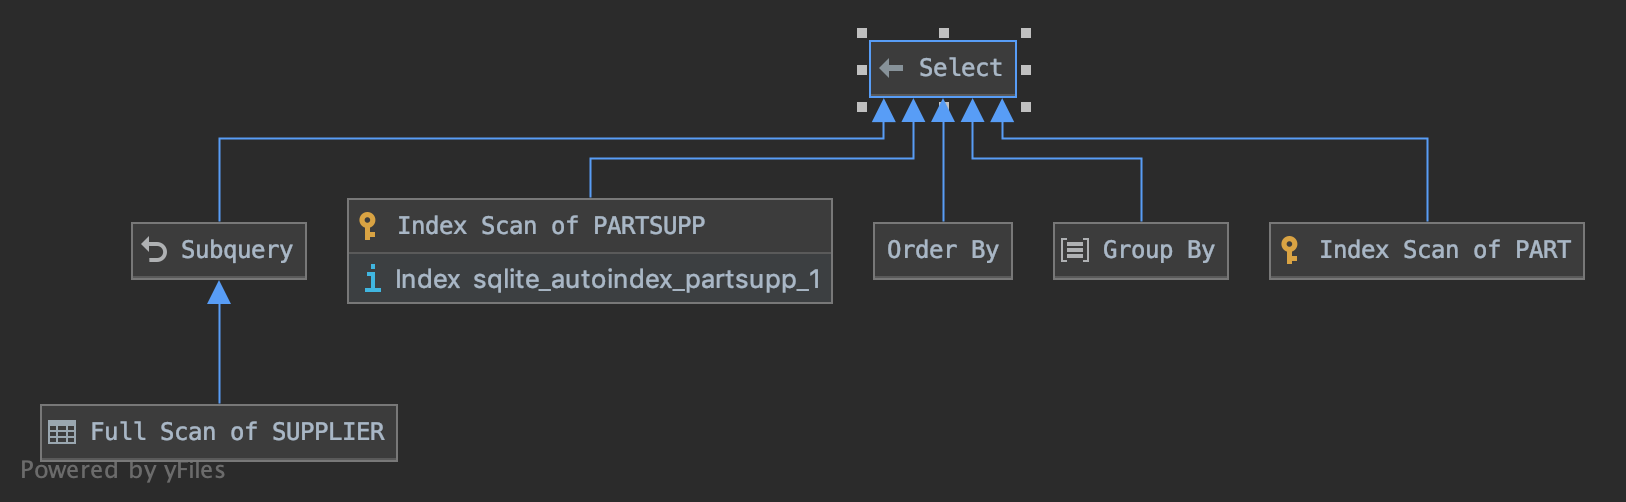
\includegraphics[width=\columnwidth]{tpch-sqllite-16}
         \caption{SQLite query plan 16 steps}
         \label{fig:tpch-sqllite-16}
     \end{subfigure}
     \hfill
     \begin{subfigure}[b]{0.4\textwidth}
         \centering
         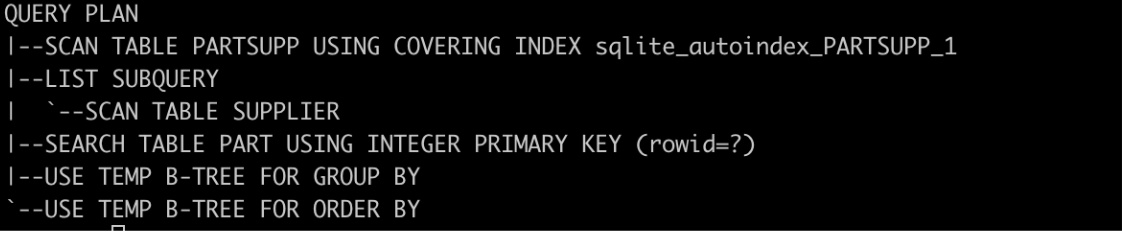
\includegraphics[width=\columnwidth]{sqlite-16-2}
         \caption{SQLite query plan 16}
         \label{fig:sqlite-16-2}
     \end{subfigure}

        \caption{SQLite plan for query 16}
        \label{fig:sqlite-16}
\end{figure*}

We now look at query 16 represented in Listing~\ref{q16} from the TPC-H benchmark suite. This is called the Parts/Supplier Relationship Query that returns how many suppliers can supply parts with given attributes. This query has almost same time for both, PostgreSQL and SQLite.

Figure~\ref{fig:tpch-postgres-16} shows the query plan generated for this query in PostgreSQL, we observe that it does a full scan of all the tables followed by some hash joins, sort, aggregate and then sort again. If we look at the query plan for SQLite in Figure~\ref{fig:sqlite-16}, we observe that it also does a scan of all the tables and execute a similar query plan. Since the query plans generated by both are significantly similar and this query does not contain the big table, LINEITEM, therefore the scans take similar time even though SQLite does an index scan. All this adds up to almost same time for this particular query in both the databases.\\

\begin{minipage}{\linewidth}
\begin{lstlisting}[breaklines=true, numbers=none, label=q16, caption=Query 16]
select p_brand, p_type, p_size, count(distinct ps_suppkey) as supplier_cnt
from partsupp, part
where p_partkey = ps_partkey
and p_brand <> '[BRAND]'
and p_type not like '[TYPE]%'
and p_size in ([SIZE1], [SIZE2], [SIZE3], [SIZE4], [SIZE5], [SIZE6], [SIZE7], [SIZE8])
and ps_suppkey not in (
select s_suppkey
from supplier
where
s_comment like '%Customer%Complaints%'
)
group by p_brand, p_type, p_size
order by supplier_cnt desc, p_brand, p_type, p_size;;
\end{lstlisting}
\end{minipage}



%\fig{width=\columnwidth}{tpch-sqllite-16}{\textmd{TPCH result}}{fig:tpch-sqllite-16}



\subsubsection{PostgreSQL faster}
\fig{width=\columnwidth}{tpch-postgres-9}{\textmd{PostgreSQL plan for query 9}}{fig:tpch-postgres-9}

\begin{figure*}[ht]
\centering
     \begin{subfigure}[b]{0.4\textwidth}
         \centering
         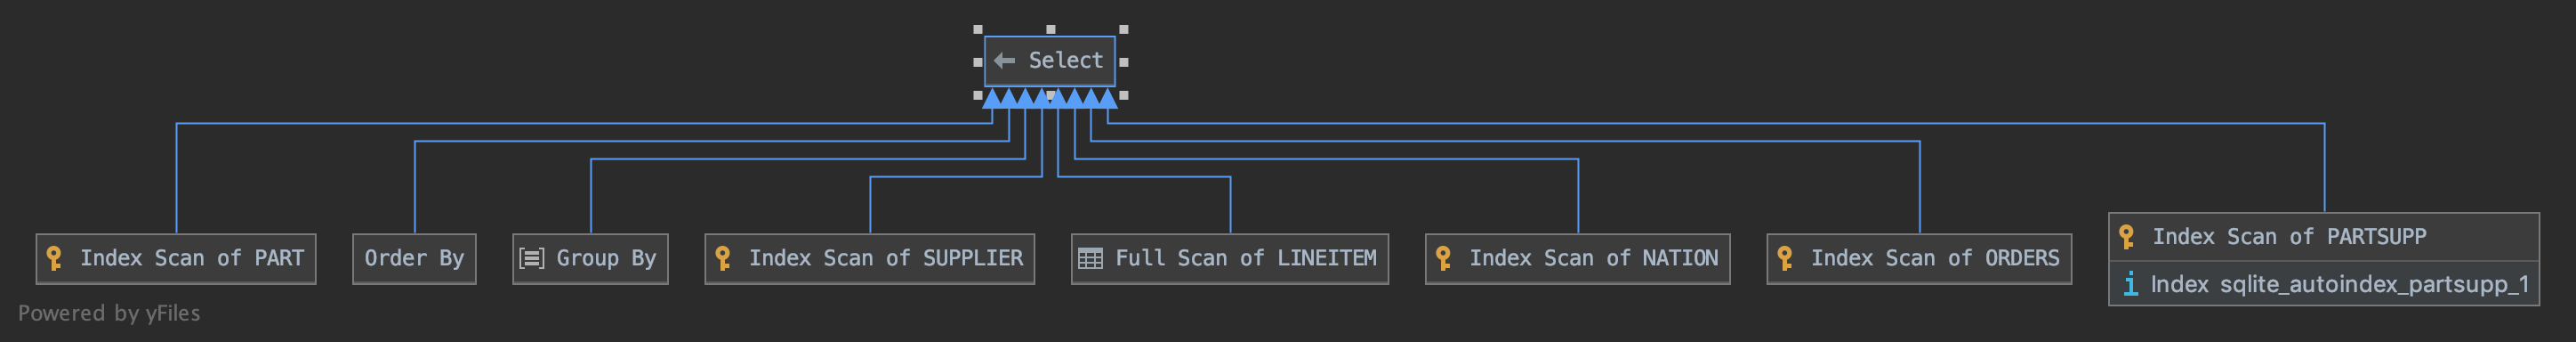
\includegraphics[width=\columnwidth]{tpch-sqllite-9}
         \caption{SQLite query plan 9 steps}
         \label{fig:tpch-sqllite-9}
     \end{subfigure}
     \hfill
     \begin{subfigure}[b]{0.4\textwidth}
         \centering
         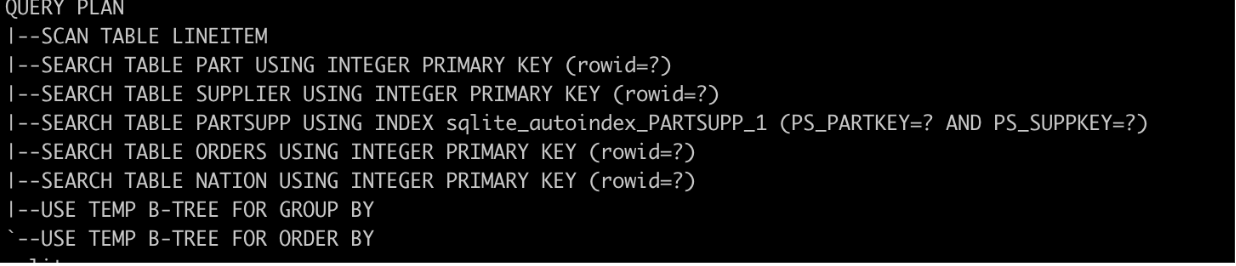
\includegraphics[width=\columnwidth]{sqlite-9-2}
         \caption{SQLite query plan 9}
         \label{fig:sqlite-9-2}
     \end{subfigure}

        \caption{SQLite plan for query 9}
        \label{fig:sqlite-9}
\end{figure*}
%\fig{width=\columnwidth}{tpch-sqllite-9}{\textmd{TPCH result}}{fig:tpch-sqllite-9}
Query 9 shown in Listing~\ref{q9} called the Product Type Profit Measure Query determines how much profit is made on a given line of parts, broken out by supplier nation and year. This query takes longer execution time SQLite.

Figure~\ref{fig:tpch-postgres-9} shows the query plan for PostgreSQL where we observe that it does full scan of all the tables followed by hash join and aggregate at the end. In SQLite shown in Figure~\ref{fig:sqlite-9}, we see many index scans. We also see that this query has LINEITEM which is a big table and hence, selectivity for this particular query is very high. Therefore, index scan in this scan becomes expensive over full scan which is seen by the lower execution time for PostgreSQL.

\begin{minipage}{\linewidth}
\begin{lstlisting}[breaklines=true, numbers=none, label=q9, caption=Query 9]
select nation, o_year, sum(amount) as sum_profit
from ( select
n_name as nation,
extract(year from o_orderdate) as o_year,
l_extendedprice * (1 - l_discount) - ps_supplycost * l_quantity as amount
from part, supplier, lineitem, partsupp, orders, nation
where s_suppkey = l_suppkey
and ps_suppkey = l_suppkey
and ps_partkey = l_partkey
and p_partkey = l_partkey
and o_orderkey = l_orderkey
and s_nationkey = n_nationkey
and p_name like '%[COLOR]%'
) as profit
group by nation, o_year
order by nation, o_year desc;
\end{lstlisting}
\end{minipage}

\subsubsection{SQLite faster}

\fig{width=\columnwidth}{tpch-postgres-4}{\textmd{PostgreSQL plan for query 4}}{fig:pgsql-4}

\begin{figure*}[ht]
\centering
     \begin{subfigure}[b]{0.4\textwidth}
         \centering
         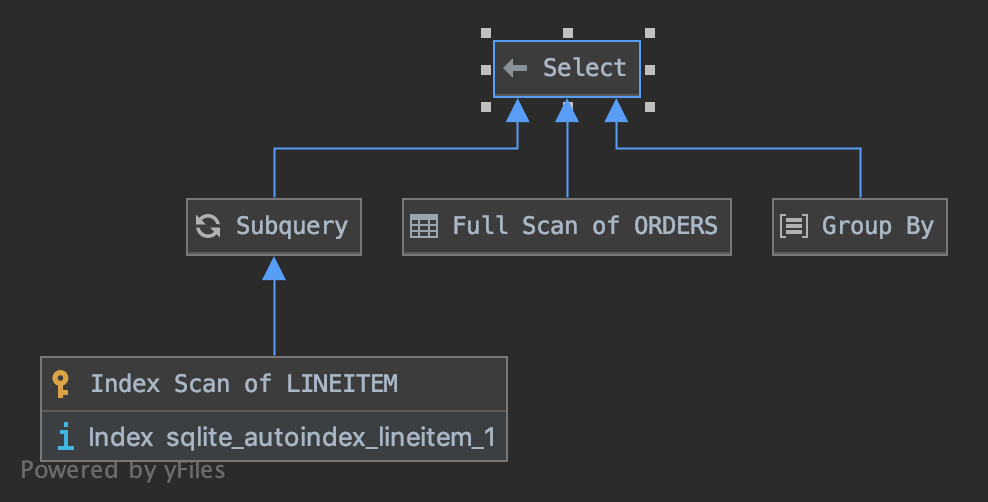
\includegraphics[width=\columnwidth]{tpch-sqllite-4}
         \caption{SQLite query plan 4 steps}
         \label{fig:tpch-sqllite-4}
     \end{subfigure}
     \hfill
     \begin{subfigure}[b]{0.4\textwidth}
         \centering
         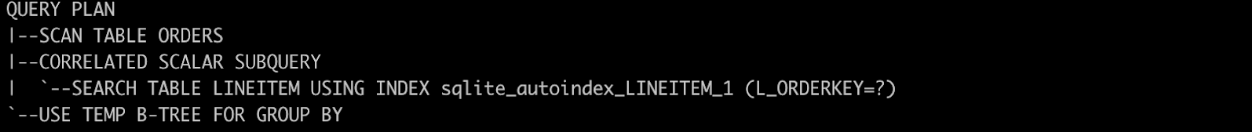
\includegraphics[width=\columnwidth]{sqlite-4-2}
         \caption{SQLite query plan 4}
         \label{fig:sqlite-4-2}
     \end{subfigure}

        \caption{SQLite plan for query 4}
        \label{fig:sqlite-4}
\end{figure*}
%\fig{width=\columnwidth}{tpch-sqllite-4}{\textmd{TPCH result}}{fig:tpch-sqllite-4}
Query 4 shown in Listing~\ref{q4} is called Order Priority Checking Query which finds how well the order priority system is working and gives an assessment of customer satisfaction. This query runs faster in SQLite.

The query plan for PostgreSQL is shown in Figure~\ref{fig:pgsql-4} and SQLite is shown in Figure~\ref{fig:sqlite-4}. This query has an inner query which is called a correlated subquery~\cite{ref:sqlite1} which depends on the outer query. The selectivity of this query is around 3\%. In case of PostgreSQL we observe that it does a full scan of all the tables whereas SQLite uses an index scan. In queries where selectivity is low, index scan is faster, therefore, we see that SQLite performs better than PostgreSQL. Since the table in question is Lineitem table which occupies 750 MB on disk out of 1GB of the entire TPC-H database, the effects seem more significant in this query than the others.\\

\begin{minipage}{\linewidth}
\begin{lstlisting}[breaklines=true, numbers=none, label=q4, caption=Query 4]
select o_orderpriority, count(*) as order_count
from orders
where o_orderdate >= date '[DATE]'
and o_orderdate < date '[DATE]' + interval '3' month
and exists (
select * from lineitem where l_orderkey = o_orderkey and l_commitdate < l_receiptdate
) group by o_orderpriority, order by, o_orderpriority;
\end{lstlisting}
\end{minipage}






